
%% bare_conf.tex
%% V1.4b
%% 2015/08/26
%% by Michael Shell
%% See:
%% http://www.michaelshell.org/
%% for current contact information.
%%
%% This is a skeleton file demonstrating the use of IEEEtran.cls
%% (requires IEEEtran.cls version 1.8b or later) with an IEEE
%% conference paper.
%%
%% Support sites:
%% http://www.michaelshell.org/tex/ieeetran/
%% http://www.ctan.org/pkg/ieeetran
%% and
%% http://www.ieee.org/

%%*************************************************************************
%% Legal Notice:
%% This code is offered as-is without any warranty either expressed or
%% implied; without even the implied warranty of MERCHANTABILITY or
%% FITNESS FOR A PARTICULAR PURPOSE! 
%% User assumes all risk.
%% In no event shall the IEEE or any contributor to this code be liable for
%% any damages or losses, including, but not limited to, incidental,
%% consequential, or any other damages, resulting from the use or misuse
%% of any information contained here.
%%
%% All comments are the opinions of their respective authors and are not
%% necessarily endorsed by the IEEE.
%%
%% This work is distributed under the LaTeX Project Public License (LPPL)
%% ( http://www.latex-project.org/ ) version 1.3, and may be freely used,
%% distributed and modified. A copy of the LPPL, version 1.3, is included
%% in the base LaTeX documentation of all distributions of LaTeX released
%% 2003/12/01 or later.
%% Retain all contribution notices and credits.
%% ** Modified files should be clearly indicated as such, including  **
%% ** renaming them and changing author support contact information. **
%%*************************************************************************


% *** Authors should verify (and, if needed, correct) their LaTeX system  ***
% *** with the testflow diagnostic prior to trusting their LaTeX platform ***
% *** with production work. The IEEE's font choices and paper sizes can   ***
% *** trigger bugs that do not appear when using other class files.       ***                          ***
% The testflow support page is at:
% http://www.michaelshell.org/tex/testflow/



\documentclass[conference]{IEEEtran}
% Some Computer Society conferences also require the compsoc mode option,
% but others use the standard conference format.
%
% If IEEEtran.cls has not been installed into the LaTeX system files,
% manually specify the path to it like:
% \documentclass[conference]{../sty/IEEEtran}




% Some very useful LaTeX packages include:
% (uncomment the ones you want to load)


% *** MISC UTILITY PACKAGES ***
%
%\usepackage{ifpdf}
% Heiko Oberdiek's ifpdf.sty is very useful if you need conditional
% compilation based on whether the output is pdf or dvi.
% usage:
% \ifpdf
%   % pdf code
% \else
%   % dvi code
% \fi
% The latest version of ifpdf.sty can be obtained from:
% http://www.ctan.org/pkg/ifpdf
% Also, note that IEEEtran.cls V1.7 and later provides a builtin
% \ifCLASSINFOpdf conditional that works the same way.
% When switching from latex to pdflatex and vice-versa, the compiler may
% have to be run twice to clear warning/error messages.






% *** CITATION PACKAGES ***
%
%\usepackage{cite}
% cite.sty was written by Donald Arseneau
% V1.6 and later of IEEEtran pre-defines the format of the cite.sty package
% \cite{} output to follow that of the IEEE. Loading the cite package will
% result in citation numbers being automatically sorted and properly
% "compressed/ranged". e.g., [1], [9], [2], [7], [5], [6] without using
% cite.sty will become [1], [2], [5]--[7], [9] using cite.sty. cite.sty's
% \cite will automatically add leading space, if needed. Use cite.sty's
% noadjust option (cite.sty V3.8 and later) if you want to turn this off
% such as if a citation ever needs to be enclosed in parenthesis.
% cite.sty is already installed on most LaTeX systems. Be sure and use
% version 5.0 (2009-03-20) and later if using hyperref.sty.
% The latest version can be obtained at:
% http://www.ctan.org/pkg/cite
% The documentation is contained in the cite.sty file itself.






% *** GRAPHICS RELATED PACKAGES ***
%
\ifCLASSINFOpdf
  % \usepackage[pdftex]{graphicx}
  % declare the path(s) where your graphic files are
  % \graphicspath{{../pdf/}{../jpeg/}}
  % and their extensions so you won't have to specify these with
  % every instance of \includegraphics
  % \DeclareGraphicsExtensions{.pdf,.jpeg,.png}
\else
  % or other class option (dvipsone, dvipdf, if not using dvips). graphicx
  % will default to the driver specified in the system graphics.cfg if no
  % driver is specified.
  % \usepackage[dvips]{graphicx}
  % declare the path(s) where your graphic files are
  % \graphicspath{{../eps/}}
  % and their extensions so you won't have to specify these with
  % every instance of \includegraphics
  % \DeclareGraphicsExtensions{.eps}
\fi
% graphicx was written by David Carlisle and Sebastian Rahtz. It is
% required if you want graphics, photos, etc. graphicx.sty is already
% installed on most LaTeX systems. The latest version and documentation
% can be obtained at: 
% http://www.ctan.org/pkg/graphicx
% Another good source of documentation is "Using Imported Graphics in
% LaTeX2e" by Keith Reckdahl which can be found at:
% http://www.ctan.org/pkg/epslatex
%
% latex, and pdflatex in dvi mode, support graphics in encapsulated
% postscript (.eps) format. pdflatex in pdf mode supports graphics
% in .pdf, .jpeg, .png and .mps (metapost) formats. Users should ensure
% that all non-photo figures use a vector format (.eps, .pdf, .mps) and
% not a bitmapped formats (.jpeg, .png). The IEEE frowns on bitmapped formats
% which can result in "jaggedy"/blurry rendering of lines and letters as
% well as large increases in file sizes.
%
% You can find documentation about the pdfTeX application at:
% http://www.tug.org/applications/pdftex





% *** MATH PACKAGES ***
%
%\usepackage{amsmath}
% A popular package from the American Mathematical Society that provides
% many useful and powerful commands for dealing with mathematics.
%
% Note that the amsmath package sets \interdisplaylinepenalty to 10000
% thus preventing page breaks from occurring within multiline equations. Use:
%\interdisplaylinepenalty=2500
% after loading amsmath to restore such page breaks as IEEEtran.cls normally
% does. amsmath.sty is already installed on most LaTeX systems. The latest
% version and documentation can be obtained at:
% http://www.ctan.org/pkg/amsmath





% *** SPECIALIZED LIST PACKAGES ***
%
%\usepackage{algorithmic}
% algorithmic.sty was written by Peter Williams and Rogerio Brito.
% This package provides an algorithmic environment fo describing algorithms.
% You can use the algorithmic environment in-text or within a figure
% environment to provide for a floating algorithm. Do NOT use the algorithm
% floating environment provided by algorithm.sty (by the same authors) or
% algorithm2e.sty (by Christophe Fiorio) as the IEEE does not use dedicated
% algorithm float types and packages that provide these will not provide
% correct IEEE style captions. The latest version and documentation of
% algorithmic.sty can be obtained at:
% http://www.ctan.org/pkg/algorithms
% Also of interest may be the (relatively newer and more customizable)
% algorithmicx.sty package by Szasz Janos:
% http://www.ctan.org/pkg/algorithmicx




% *** ALIGNMENT PACKAGES ***
%
%\usepackage{array}
% Frank Mittelbach's and David Carlisle's array.sty patches and improves
% the standard LaTeX2e array and tabular environments to provide better
% appearance and additional user controls. As the default LaTeX2e table
% generation code is lacking to the point of almost being broken with
% respect to the quality of the end results, all users are strongly
% advised to use an enhanced (at the very least that provided by array.sty)
% set of table tools. array.sty is already installed on most systems. The
% latest version and documentation can be obtained at:
% http://www.ctan.org/pkg/array


% IEEEtran contains the IEEEeqnarray family of commands that can be used to
% generate multiline equations as well as matrices, tables, etc., of high
% quality.




% *** SUBFIGURE PACKAGES ***
%\ifCLASSOPTIONcompsoc
%  \usepackage[caption=false,font=normalsize,labelfont=sf,textfont=sf]{subfig}
%\else
%  \usepackage[caption=false,font=footnotesize]{subfig}
%\fi
% subfig.sty, written by Steven Douglas Cochran, is the modern replacement
% for subfigure.sty, the latter of which is no longer maintained and is
% incompatible with some LaTeX packages including fixltx2e. However,
% subfig.sty requires and automatically loads Axel Sommerfeldt's caption.sty
% which will override IEEEtran.cls' handling of captions and this will result
% in non-IEEE style figure/table captions. To prevent this problem, be sure
% and invoke subfig.sty's "caption=false" package option (available since
% subfig.sty version 1.3, 2005/06/28) as this is will preserve IEEEtran.cls
% handling of captions.
% Note that the Computer Society format requires a larger sans serif font
% than the serif footnote size font used in traditional IEEE formatting
% and thus the need to invoke different subfig.sty package options depending
% on whether compsoc mode has been enabled.
%
% The latest version and documentation of subfig.sty can be obtained at:
% http://www.ctan.org/pkg/subfig




% *** FLOAT PACKAGES ***
%
%\usepackage{fixltx2e}
% fixltx2e, the successor to the earlier fix2col.sty, was written by
% Frank Mittelbach and David Carlisle. This package corrects a few problems
% in the LaTeX2e kernel, the most notable of which is that in current
% LaTeX2e releases, the ordering of single and double column floats is not
% guaranteed to be preserved. Thus, an unpatched LaTeX2e can allow a
% single column figure to be placed prior to an earlier double column
% figure.
% Be aware that LaTeX2e kernels dated 2015 and later have fixltx2e.sty's
% corrections already built into the system in which case a warning will
% be issued if an attempt is made to load fixltx2e.sty as it is no longer
% needed.
% The latest version and documentation can be found at:
% http://www.ctan.org/pkg/fixltx2e


%\usepackage{stfloats}
% stfloats.sty was written by Sigitas Tolusis. This package gives LaTeX2e
% the ability to do double column floats at the bottom of the page as well
% as the top. (e.g., "\begin{figure*}[!b]" is not normally possible in
% LaTeX2e). It also provides a command:
%\fnbelowfloat
% to enable the placement of footnotes below bottom floats (the standard
% LaTeX2e kernel puts them above bottom floats). This is an invasive package
% which rewrites many portions of the LaTeX2e float routines. It may not work
% with other packages that modify the LaTeX2e float routines. The latest
% version and documentation can be obtained at:
% http://www.ctan.org/pkg/stfloats
% Do not use the stfloats baselinefloat ability as the IEEE does not allow
% \baselineskip to stretch. Authors submitting work to the IEEE should note
% that the IEEE rarely uses double column equations and that authors should try
% to avoid such use. Do not be tempted to use the cuted.sty or midfloat.sty
% packages (also by Sigitas Tolusis) as the IEEE does not format its papers in
% such ways.
% Do not attempt to use stfloats with fixltx2e as they are incompatible.
% Instead, use Morten Hogholm'a dblfloatfix which combines the features
% of both fixltx2e and stfloats:
%
% \usepackage{dblfloatfix}
% The latest version can be found at:
% http://www.ctan.org/pkg/dblfloatfix




% *** PDF, URL AND HYPERLINK PACKAGES ***
%
%\usepackage{url}
% url.sty was written by Donald Arseneau. It provides better support for
% handling and breaking URLs. url.sty is already installed on most LaTeX
% systems. The latest version and documentation can be obtained at:
% http://www.ctan.org/pkg/url
% Basically, \url{my_url_here}.




% *** Do not adjust lengths that control margins, column widths, etc. ***
% *** Do not use packages that alter fonts (such as pslatex).         ***
% There should be no need to do such things with IEEEtran.cls V1.6 and later.
% (Unless specifically asked to do so by the journal or conference you plan
% to submit to, of course. )


% correct bad hyphenation here
\hyphenation{op-tical net-works semi-conduc-tor}


\begin{document}
%
% paper title
% Titles are generally capitalized except for words such as a, an, and, as,
% at, but, by, for, in, nor, of, on, or, the, to and up, which are usually
% not capitalized unless they are the first or last word of the title.
% Linebreaks \\ can be used within to get better formatting as desired.
% Do not put math or special symbols in the title.
\title{Report for CSAW ESC 2017}


% author names and affiliations
% use a multiple column layout for up to three different
% affiliations
\author{\IEEEauthorblockN{Chenglu Jin, Saeed Valizadeh, Mason Ginter and Marten van Dijk}
\IEEEauthorblockA{University of Connecticut\\
Email: \{chenglu.jin, saeed.val, mason.ginter, marten.van\_dijk\}@uconn.edu}
}

% conference papers do not typically use \thanks and this command
% is locked out in conference mode. If really needed, such as for
% the acknowledgment of grants, issue a \IEEEoverridecommandlockouts
% after \documentclass

% for over three affiliations, or if they all won't fit within the width
% of the page, use this alternative format:
% 
%\author{\IEEEauthorblockN{Michael Shell\IEEEauthorrefmark{1},
%Homer Simpson\IEEEauthorrefmark{2},
%James Kirk\IEEEauthorrefmark{3}, 
%Montgomery Scott\IEEEauthorrefmark{3} and
%Eldon Tyrell\IEEEauthorrefmark{4}}
%\IEEEauthorblockA{\IEEEauthorrefmark{1}School of Electrical and Computer Engineering\\
%Georgia Institute of Technology,
%Atlanta, Georgia 30332--0250\\ Email: see http://www.michaelshell.org/contact.html}
%\IEEEauthorblockA{\IEEEauthorrefmark{2}Twentieth Century Fox, Springfield, USA\\
%Email: homer@thesimpsons.com}
%\IEEEauthorblockA{\IEEEauthorrefmark{3}Starfleet Academy, San Francisco, California 96678-2391\\
%Telephone: (800) 555--1212, Fax: (888) 555--1212}
%\IEEEauthorblockA{\IEEEauthorrefmark{4}Tyrell Inc., 123 Replicant Street, Los Angeles, California 90210--4321}}




% use for special paper notices
%\IEEEspecialpapernotice{(Invited Paper)}




% make the title area
\maketitle

\begin{abstract}
In this report, we briefly explain our defense strategy in order to secure Programmable Logic Controllers (PLCs).
\end{abstract}



\section{Introduction}

A host-based intrusion detection (HIDS) is commonly used for monitoring specific activities and characteristics of a single device by means of software or appliance-based components known as agents \cite{ids}. A HIDS is able to provide system level checks (e.g. file integrity checking, log analysis, rootkit detection, etc.), detailed logging information, encrypted communications monitoring, and very small false positives' rates due to an ample knowledge of the configurations and characteristics of the host under its watch, in addition to having a thorough operating sytem level access to communication streams and sessions. 

We have looked into different possible security proposals which could potentially be used for this project, i.e., securing the PLCs. Amongst available works, we found \cite{simbiote} and \cite{pillarbox} more relevant and applicable for this project. \cite{simbiote} proposes a host-based defense mechanism called Symbiotic Embedded
Machines or ``SEM'' which adds an intrusion detection functionality to the firmware layer of an embedded system.  As the SEM structure
operates alongside the native OS of the embedded device and not within it, it can
inject generic defensive payloads into the target device regardless of it's original
hardware or software. On the other hand, \cite{pillarbox} introduces an interesting tool called PillarBox for the purpose of securely relaying Security Analytics Sources (SASs) data to combat an adversary taking advantage of an advanced malware who can undetectably
suppress or tamper with SAS messages in order to hide attack evidence and disrupt intrusion detection. Pillarbox provides two unique features: 
\begin{itemize}
	\item Integrity: By securing SAS data against tampering, even when such data is buffered on a compromised host within an adversarially controlled network.
	\item Stealthiness: By concealing SAS data, alert-generation activity and potentially even alerting rules on a compromised
	host, thus hiding select SAS alerting actions from an adversary.
\end{itemize}

 In this regard, in this project, by using the idea introduced in \cite{pillarbox},  we implemented a very lightweight HIDS module on the OpenPLC framework in order to keep track of input/output operations on the device. To locate signs of likely security related incidents, the HIDS's agent installed on each PLC, which we call it the \emph{Snapshotter}, logs all the events on the controller (more specifically, input/output operations). Then the Snapshotter sends the snapshot, which is indeed the log of operations happening on the PLC at a specific time,  in a \emph{stealthy and secure way} to a server periodically for the purpose of anaylsis and intrusion detection. 
 
On the other hand, the implemented server first checks the integrity of the log itself (in case, the attacker has already compromised the device). Moreover, it has a predefined set of acceptable input/output pairs for each device and checks and the validity of the operations happening on the controller. If any of the previous incidents happens, i.e., whether the log's integrity check fails, or an operation is detected as invalid, a flag will be raised and an intrusion is indeed captured\footnote{Assuming no errors in the controller functionality itself. Note that, even if there is an error in the PLC functionality, our proposed method can capture it as well with the same procedure}. The server takes proper actions consequently which could be terminating the controller, revoking it from the network, or even recovering it to a clean/safe state.

In order to have tamper-resistant logs, we use a forward-secure integrity protection mechanism in which the controller generate new keys after every alert generation and delete keys immediately after use \cite{pillarbox}. For the operation validation purposes, the server actually traces deviations from predefined acceptable normal profile activities of the input/output operations. Such profile activities could be generated based on the specific applications that the PLC is being used for. As an example, lets say the adversary somehow has root access to the system, and can generate some sort of malicious input/output pairs, such activity can be captured by our proposed method, since the adversary can not tamper the logs and the server will restore the PLC into its normal state by uploading a known valid logic into the PLC.
%what are proper server responses in case of an intrusion???

Our defense mechanism can be summarized in security related information gathering and secure logging, sending the logs to a server for the purpose of analysis, incident identification and taking effective actions by the server to foil such incidents. We explain each part in more detail in the following sections.




\section{Introduction}

A host-based intrusion detection (HIDS) is commonly used for monitoring specific activities and characteristics of a single device by means of software or appliance-based components known as agents. In this regard, in this project, we implemented a very lightweight HIDS module on the OpenPLC framework in order to keep track of input/output operations on the device.

To locate signs of likely security related incidents, the HIDS's agent, which we call it the \emph{snapshotter} agent, essentially, takes a snapshot of the input/output operations
happening on each PLC and sends them \emph{in a stealthy secure way} to a server periodically. Then, the server 

To locate signs of likely security related incidents, this agent, which is installed on each plc, logs all the events on the controller (more specifically, input/output operations) and sends the logs to a server periodically for the purpose of anaylsis and intrusion detection. 

On the other hand, the implemented server has a predefined set of acceptable input/output pairs for each device and checks the integrity of the log itself (in case, the attacker has already compromised the device) and the validity of the operations happening on the controller. If any of the previous incidents happen, i.e., whether the log's integrity check fails, or an operation is detected as invalid, a flag will be raised and an intrusion is indeed captured\footnote{Assuming no errors in the controller functionality itself. Note that, even if there is error in the PLC functionality, our proposed method can capture it as well with same procedure}. The server takes proper actions consequently which could be terminating the controller, revoking it from the network, or even recovering it to a previous clean/safe state.

For the log integrity checking feature, the server actually 

For the operation validation purposes, the server actually traces deviations from predefined normal profile activities/behaviors of the input/output operations. Such profile activities could be generated based on the specific applications that the PLC is being used for. (see the comments in tex file)
%what are proper server responses in case of an intrusion???

Our defense mechanism can be summarized in security related information gathering and logging, incident identification, and taking effective actions to foil such incidents.






\section{Proposed Defense Scheme}

\begin{figure*}[h]
  \centering
    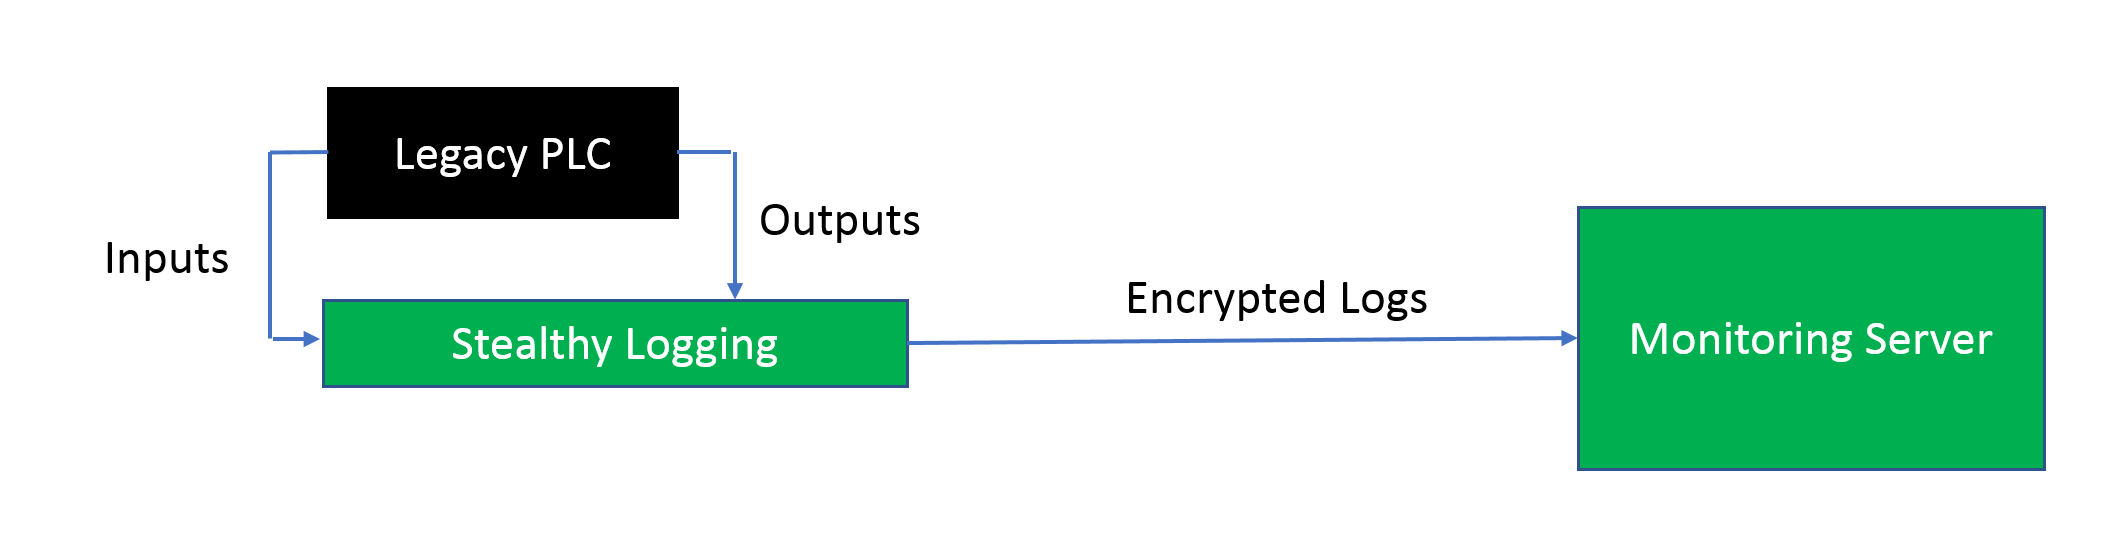
\includegraphics[width=\textwidth]{figs/legacy_system}
    \caption{Our proposed system with legacy PLCs.}
    \label{fig:legacy}
\end{figure*}

\begin{figure*}[h]
  \centering
    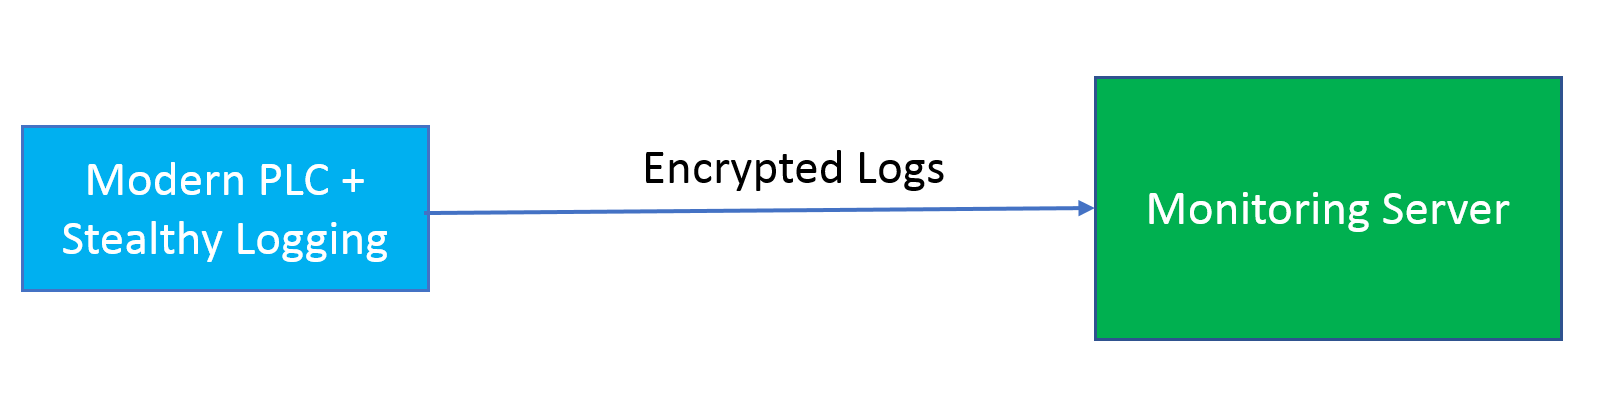
\includegraphics[width=0.8\textwidth]{figs/modern_system}
    \caption{Our proposed system with modern PLCs.}
    \label{fig:modern}
\end{figure*}


%A host-based intrusion detection (HIDS) is commonly used for monitoring specific activities and characteristics of a single device by means of software or appliance-based components known as agents. In this regard, 
In this project, we implement a very lightweight HIDS module in the OpenPLC framework~\cite{alves2014openplc} in order to keep track of input/output operations on the device.

To locate the intrusions, the \emph{snapshotter} agent, essentially, takes a snapshot of the input/output values together with the current time stamps on each PLC, encrypts the log, and sends them \emph{in a stealthy secure way} to a server periodically. Forward security is achieved in the key management of the encryption key. Next key is updated to the hash of the current key after each encryption. Therefore, even the adversary compromised the device completely, meaning that the encryption key is also exposed to the adversary, he is still not able to tell from the previous encrypted logs that whether he is caught by the intrusion detection systems or not.   

Upon receiving the reports from PLCs, the server can use the received input and known PLC logic to simulate the expected output of the PLC. If the received PLC output does not match with the expected (simulated) output, then the server will conclude that this PLC has been compromised, so it should be restarted and restored to a clean state/reprogrammed by a correct logic program. Of course, for a specific application, the server can have a predefined set of acceptable input/output pairs for each device. This will reduce the computation of the server side. Besides the input/output behaviors, the integrity of the log can be checked at the server, in case that the attacker has already compromised the device.

Our defense mechanism can be summarized in security related information gathering and logging, incident identification, and taking effective actions to foil such incidents.

This solution has five features that make our proposed scheme very suitable to the intrusion detection for PLCs:

\begin{enumerate}
\item We can guarantee the integrity of the log generated by each PLCs, because we are able to verify its integrity at the server side, and we can detect any dropped package in the communication.  

\item The log is sent in a stealthy way, such that the attacker is not able to tell whether he gets detected or not. This gives more advantages to the defenders to record more behaviors of the attackers, which can be used for further investigations.  

\item This approach requires no redundant PLCs for detecting an intrusion, so it saves the cost of extra PLCs for implementing any intrusion detection schemes, e.g. comparing the outputs of two redundant PLCs. 

\item Our approach can be applied on any legacy PLCs, because we only record the inputs and outputs of each PLCs in the log. No internal states of the PLCs are required. 

\item Since the logic running on the PLCs is usually very simple, a powerful server can easily simulate a large number of PLCs in parallel. This makes our solution easily scalable to monitor a large number of PLCs.

\item In the scenario of an industrial control system, all the devices are connected using cables, so the connectivity of each PLC device is very well established. This will reduce the false positive of our system caused by the network delay. 

\end{enumerate} 

When our solution is implemented on the legacy PLCs, the system will be like Figure~\ref{fig:legacy}. The legacy PLCs are black boxes to us, we can only record input/output values of them and send this information as logs to the server. The advantage of applying our solution on legacy PLCs is that the PLCs and the logging mechanism are isolated from one another. An adversary, who compromise the legacy PLCs, still cannot tamper with the logging mechanism, which leads to an easy detection for the server. 

In contrast, when our logging mechanism is implemented in modern PLCs, no extra new hardware is required, and we can even record more information than simply input/output values. This will help the server know more about the status of the PLCs. But since the PLC logic are running together with the logging mechanism on the same device, compromising PLCs only means compromising the logging scheme and the encryption keys. Fortunately, our solution can maintain the security even when the encryption key is exposed to the adversary. We provide more detailed analysis in Section. IV.   

\subsection{Information Gathering}

In order to achieve the stealth logging, we suggest to use the logging mechanism in \cite{IEEEhowto:kopka}. The log has two requirements:

\begin{enumerate}
\item All the logs are encrypted, and the encryption key is updated in a forward secure key. 
\item The logs are buffered in the device itself, and is sent periodically to the server.
\end{enumerate}

The first requirement prevents the adversary, who eavesdrops the communication between the PLCs and the server, from figuring out whether the current attack is being detected or not. A forward secure key management scheme guarantees that even when the current key is compromised by the adversary, the adversary is still not able to decrypt all the encrypted logs sent before. 

The second requirement prevents the attackers from dropping all the encrypted logs that possibly record some traces of the adversary, because if the report of one device is not sent to the server on time, the server will conclude that this device has compromised by attackers.

\subsection{Incident Identification}

If any of the incidents happen, i.e., whether the log's integrity check fails, or an operation is detected as incorrect, a flag will be raised and an intrusion is indeed captured\footnote{Assuming no errors in the controller functionality itself. Note that, even if there is error in the PLC functionality, our proposed method can capture it as well with same procedure}. The server takes proper actions consequently which could be terminating the controller, revoking it from the network, or even recovering it to a previous clean/safe state.

%For the operation validation purposes, the server actually traces deviations from predefined normal profile activities/behaviors of the input/output operations. Such profile activities could be generated based on the specific applications that the PLC is being used for. (see the comments in tex file)
%what are proper server responses in case of an intrusion???
%


\subsection{Mitigation}

Once an incident has been identified, one can restart the compromised PLCs, and reprogram it to a safe/correct state/logic. If the monitoring server is not able to reset the PLC to a clean state, then a technician must be sent to physically approach the PLC and fix it. In the meanwhile, another uncompromised PLC can be deployed to replace the compromised PLC to continue the industrial process. 

\section{Implementation}

\subsection{Algorithms}

We implemented the stealthy logging mechanism in OpenPLC framework on a Raspberry Pi. The operations in one scan cycle can be described in Algorithm~\ref{logging_algo}. In OpenPLC framework, \textbf{Read\_Input} function and \textbf{Write\_Output} function has been modified to return 1 if any value changes in the current scan cycle. Therefore, only when the input or output values change, this event will be recorded in the log. A single event is encrypted and its key is updated to its hash value, such that the old key for encrypting this event will be overwritten right after each encryption. 

Since the input or output of PLC does not change very often, only reporting changes of input/output values in the log, we can significantly reduce the size of the log. For an application that requires the inputs/outputs of PLCs to be updated very frequently, we suggest to reduce reporting period or ignore some small fluctuations in the analog output.  

After a predefined reporting period is elapsed, the PLC needs to send all the buffered encrypted log to the server and empty the buffer for the next period.

\begin{algorithm}[!t]
\caption{PLC Logging}\label{logging_algo}
\begin{algorithmic}[1]
\Procedure{Logging}{$Period$}
	
	\State $EL = \{\}$
	\State $T = 0$
	\State $Event\_ID = 0$
	\State $Update = 0$
	
	\While{True} \Comment{Scan Cycle}
		\State $Update = 0$
		\State $T = T + 1$
		\State $Update = Read\_Input()$
		\State $PLC\_Logic()$
		\State $Update = Write\_Ouput()$
		\If{$Update == 1 || T \mbox{ mod } Period == 1 $}
			\State $TempLog = \{T, Input, Output, Event\_ID\}$
			\State $EL \gets $(\Call{Encrypt}{$Temp\_Log$, $Key$})
			\State $TempLog = \emptyset$ \Comment{Delete the plaintext}
			\State $Key = $\Call{Hash}{$Key$}
			\State $Event\_ID = Event\_ID + 1$
		\EndIf
		\If{$T\mbox{ mod }Period == 0$}
			\State \Call{Send}{EL}
			\State $EL = \emptyset$ \Comment{Empty the buffer}
			\State $Event\_ID = 0$
		\EndIf
	\EndWhile
\EndProcedure
\end{algorithmic}
\end{algorithm}

The algorithm on the server side works as Algorithm~\ref{server_algo}. The server waits for the incoming packet from the PLC. If the packet is not received on time, the server concludes that the PLC is compromised, we need to restart the PLC. If the server gets the packet on time, then we need to use the associated key to decode this packet and update the key stored at the server. After that, we need to check whether the decrypted data has the correct data format or not. If not, then it means the integrity of the packet has been compromised, we need to restart the PLC. If the integrity is also valid, then we need to extract the input change in this period with its time stamp. This input change and time information is applied to the PLC logic simulator, which will generate the expect output change with its time stamp. Then this expected output is compared with the output received from the PLCs. If they do not match, then the server knows that the logic running on the PLC has been maliciously modified. Therefore, it is also required to restart the PLC in this case.   

\begin{algorithm}[!t]
\caption{Server Monitoring}\label{server_algo}
\begin{algorithmic}[1]
\Procedure{Monitoring}{$Period$}
	
	\State $Alarm = False$
	\State $Last\_Rec\_T = Current\_T$
	
	\While{True}
		\While{True}
			\If {$Current\_T - Last\_Rec\_T > Period$}
				\State $Alarm = True$
				\State Break \Comment{Missing one Packet}
			\EndIf
			\If {$EL \gets$ \Call{Rec\_Packet}}
				\State $Last\_Rec\_T = Current\_T$ 
				\State Break \Comment{Receive one Packet}
			\EndIf
		\EndWhile
		\State $(L, Key) \gets $ \Call{Decrypt\_Packet}{$EL,Key$}
		\State $Alarm \gets $ \Call{Verify\_Format}{$L$}
		\State $(T', Input', Output', Event\_ID') \gets L$
		\State $(T'', Output'') \gets $ \Call{PLC\_Simulate}{$T', Input'$}
		\State $Alarm \gets $ \Call{Compare}{$T', Ouput', T'', Output''$}
		\If {Alarm}
			\State Restart PLC
		\EndIf
	\EndWhile
\EndProcedure
\end{algorithmic}
\end{algorithm}

\subsection{Implementation Details}

As cryptographic primitives, we use AES-128 and SHA-256 as the encryption algorithm and hash function respectively. The updated key is the first 16 bytes of the hash value of the previous key. The reporting period is set to 10 seconds in the prototype implementation, but it can be easily adapted to a different value if it is required by the application. 

To minimize the size of the log we sent, we design one data format to record one event (input or output change) in less than 128 bits, which can fit in one encryption block of AES. The data format is depicted in Figure~\ref{fig:data_format}. The first byte is used as an indicator of the start of one event; we set it as 0xFF. The second and third bytes are used to store the event ID in the current time period. Since the PLC is required to run on 100Hz, and we set the reporting period to be 10 seconds, the maximum of events can happen in one period is 1000. Therefore, two bytes are more than enough to represent the maximum number. The forth and fifth bytes are reserved for device ID. In total, 65536 devices are allowed to be managed by one server. The following 4 bytes are used to store the time stamp, because in OpenPLC framework, it is a 4 byte variable. The next six bytes are divided for storing digital inputs, digital outputs and analog output value respectively. Each of them takes two bytes. Since the number of digital inputs and digital outputs on a Raspberry Pi is 14 and 11. Two bytes are enough to store all the input/output pins. Also, only one analog pin can be used on a Raspberry Pi, and this value can be represented by a 16-bit value stored in 2 bytes. In the end, another byte of 0xFF is appended to indicate the end of one event log. 

\begin{figure*}[h]
  \centering
    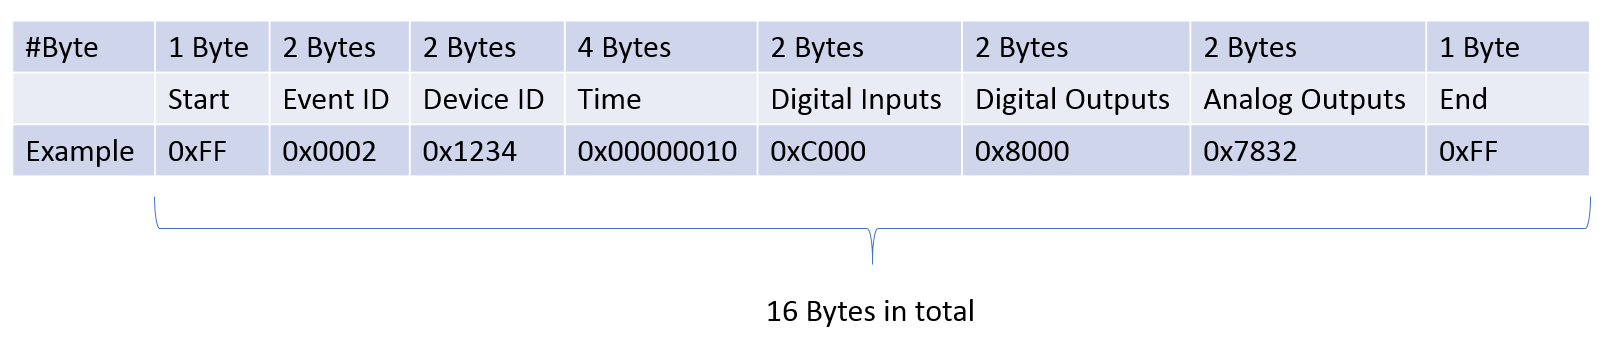
\includegraphics[width=\textwidth]{figs/data_format}
    \caption{Data format of one event in the log.}
    \label{fig:data_format}
\end{figure*}


\section{Evaluation}

In this section, we will evaluate our solution and implementation in terms of security and performance. 

\subsection{Security Analysis}

Our adversarial model is that we assume the adversary has the capability to upload malicious logic to the PLC that will generate erroneous outputs or further compromise the entire PLC. After the entire PLC is compromised, we assume the attacker can even get access to the encryption key, which will be used to encrypt the next event, together with the encrypted logs that have not been sent to the server yet. This is a very strong adversarial model for a remote attacker who is connected over the network. Only when our solution is applied to a modern PLC or OpenPLC, meaning that the PLC logic and the   When our solution is applied to the legacy PLCs, the logging mechanism is implemented outside of the legacy PLCs as another hardware layer, so a remote attacker has no way to get the key in it.  

In addition, we assume that the logging mechanism is working properly until a certain point after the compromise initiates. In other words, we assume there exist a time window that the attacker has initiated the intrusion, but the logging is still working properly. The overall timeline can be illustrated as Figure.~\ref{fig:timeline}. 

\begin{figure*}[h]
  \centering
    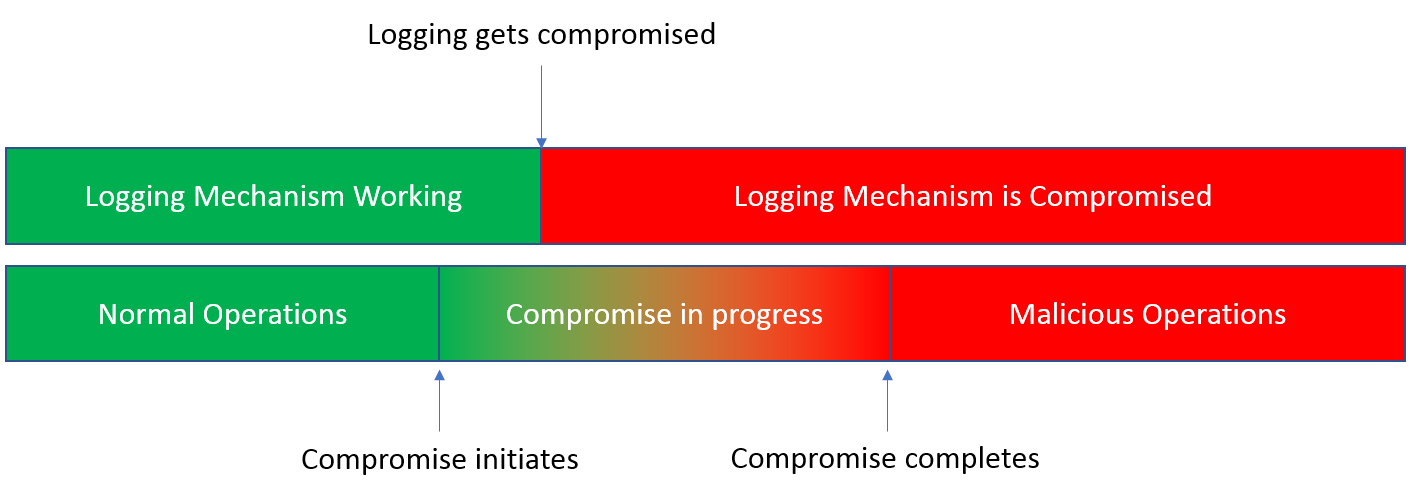
\includegraphics[width=\textwidth]{figs/timeline}
    \caption{Time line of one compromise.}
    \label{fig:timeline}
\end{figure*}

The time window between the start of a compromise and the moment that the logging failed is very critical. Essentially the logs generated in this time window tells the server that an intrusion is happening. The attacker has four different approaches to deal with this log, and all of them will lead to detection. We list all the four possible approaches below:

\begin{enumerate}
\item \textbf{Let the encrypted logs send to the server. } Since this log contains the information about intrusion, the adversary will be detected.

\item \textbf{Try to decrypt the logs.} Notice that, it is possible that the adversary compromises the device completely (i.e. knowing the current encryption key) before the log has been sent. But the previous log has already been encrypted and buffered, and the encryption key is updated in a forward secure way. The attacker has no chance to inverse the hash function and gets to know the previous encryption key. Therefore, the attacker is not able to decrypt the log, and has to send this log as it is. 

\item \textbf{Tamper with the encrypted logs.} The attacker can either send something random or replay a previous log about a clean state. Since the encryption key is updated after each event, the server with an updated key will not be able to decrypt this tampered log. Therefore, the server will also conclude that an intrusion is happening on this PLC. 

\item \textbf{Block the communication between the PLC and the server.} If the communication between the compromised PLC and the server is blocked, no log will arrive the server on time. Since the PLC is required to send the report periodically, any PLC which fails to send the log on time will be considered as compromised. 

\end{enumerate}     

To summarize, there is no way for the attackers to avoid detecting by our intrusion detection scheme. 

\subsection{Sensitivity of Detection}

Since our solution requires the logs from PLCs to be sent periodically, it is possible for the server to have a detection latency no larger than a reporting period. Hence, when we select the parameter of reporting period, we need to consider this detection latency as well. 
   
\subsection{Performance Overhead}

We run the simple helloworld logic on the OpenPLC platform. It takes 10.375 microseconds for the original OpenPLC implementation to execute all the program in one scan cycle. Using the original OpenPLC implementation as the baseline design, we measured the performance overhead of our system when it has one event in one period, meaning that no input/output changes in this period. The overhead is 21.6\%, assuming each period has 1000 scan cycles. When more events happening, we will have more performance overhead. For examples, when four events happened in one period, the overhead will become 33.0\%.   

  


\section{Future Works}

In the future, we can implement this scheme to a complete industrial control network, which has a real powerful server connected to. This can help us study how much this scheme can be scale in practice, due to the constraints on the network bandwidth or a certain application. 

Also, we need to investigate a more efficient mitigation strategy, that affects the real industrial process as little as possible.  


\section{Conclusion}

In this project, we implemented stealthy logging mechanism on the PLCs, and the server also runs the monitoring program. 



% For peer review papers, you can put extra information on the cover
% page as needed:
% \ifCLASSOPTIONpeerreview
% \begin{center} \bfseries EDICS Category: 3-BBND \end{center}
% \fi
%
% For peerreview papers, this IEEEtran command inserts a page break and
% creates the second title. It will be ignored for other modes.
\IEEEpeerreviewmaketitle



\section{Implemented Defense strategy}

A host-based intrusion detection (HIDS) is commonly used for monitoring specific activities and characteristics of a single device by means of software or appliance-based components known as agents. In this regard, in this project, we implemented a very lightweight HIDS module on the OpenPLC framework in order to keep track of input/output operations on the device.

To locate signs of likely security related incidents, the HIDS's agent, which we call it the \emph{snapshotter} agent, essentially, takes a snapshot of the input/output operations
happening on each PLC and sends them \emph{in a stealthy secure way} to a server periodically. Then, the server 

To locate signs of likely security related incidents, this agent, which is installed on each plc, logs all the events on the controller (more specifically, input/output operations) and sends the logs to a server periodically for the purpose of anaylsis and intrusion detection. 

On the other hand, the implemented server has a predefined set of acceptable input/output pairs for each device and checks the integrity of the log itself (in case, the attacker has already compromised the device) and the validity of the operations happening on the controller. If any of the previous incidents happen, i.e., whether the log's integrity check fails, or an operation is detected as invalid, a flag will be raised and an intrusion is indeed captured\footnote{Assuming no errors in the controller functionality itself. Note that, even if there is error in the PLC functionality, our proposed method can capture it as well with same procedure}. The server takes proper actions consequently which could be terminating the controller, revoking it from the network, or even recovering it to a previous clean/safe state.

For the log integrity checking feature, the server actually 

For the operation validation purposes, the server actually traces deviations from predefined normal profile activities/behaviors of the input/output operations. Such profile activities could be generated based on the specific applications that the PLC is being used for. (see the comments in tex file)
%what are proper server responses in case of an intrusion???

Our defense mechanism can be summarized in security related information gathering and logging, incident identification, and taking effective actions to foil such incidents.






%\subsection{Subsection Heading Here}
%Subsection text here.


%\subsubsection{Subsubsection Heading Here}
%Subsubsection text here.


% An example of a floating figure using the graphicx package.
% Note that \label must occur AFTER (or within) \caption.
% For figures, \caption should occur after the \includegraphics.
% Note that IEEEtran v1.7 and later has special internal code that
% is designed to preserve the operation of \label within \caption
% even when the captionsoff option is in effect. However, because
% of issues like this, it may be the safest practice to put all your
% \label just after \caption rather than within \caption{}.
%
% Reminder: the "draftcls" or "draftclsnofoot", not "draft", class
% option should be used if it is desired that the figures are to be
% displayed while in draft mode.
%
%\begin{figure}[!t]
%\centering
%\includegraphics[width=2.5in]{myfigure}
% where an .eps filename suffix will be assumed under latex, 
% and a .pdf suffix will be assumed for pdflatex; or what has been declared
% via \DeclareGraphicsExtensions.
%\caption{Simulation results for the network.}
%\label{fig_sim}
%\end{figure}

% Note that the IEEE typically puts floats only at the top, even when this
% results in a large percentage of a column being occupied by floats.


% An example of a double column floating figure using two subfigures.
% (The subfig.sty package must be loaded for this to work.)
% The subfigure \label commands are set within each subfloat command,
% and the \label for the overall figure must come after \caption.
% \hfil is used as a separator to get equal spacing.
% Watch out that the combined width of all the subfigures on a 
% line do not exceed the text width or a line break will occur.
%
%\begin{figure*}[!t]
%\centering
%\subfloat[Case I]{\includegraphics[width=2.5in]{box}%
%\label{fig_first_case}}
%\hfil
%\subfloat[Case II]{\includegraphics[width=2.5in]{box}%
%\label{fig_second_case}}
%\caption{Simulation results for the network.}
%\label{fig_sim}
%\end{figure*}
%
% Note that often IEEE papers with subfigures do not employ subfigure
% captions (using the optional argument to \subfloat[]), but instead will
% reference/describe all of them (a), (b), etc., within the main caption.
% Be aware that for subfig.sty to generate the (a), (b), etc., subfigure
% labels, the optional argument to \subfloat must be present. If a
% subcaption is not desired, just leave its contents blank,
% e.g., \subfloat[].


% An example of a floating table. Note that, for IEEE style tables, the
% \caption command should come BEFORE the table and, given that table
% captions serve much like titles, are usually capitalized except for words
% such as a, an, and, as, at, but, by, for, in, nor, of, on, or, the, to
% and up, which are usually not capitalized unless they are the first or
% last word of the caption. Table text will default to \footnotesize as
% the IEEE normally uses this smaller font for tables.
% The \label must come after \caption as always.
%
%\begin{table}[!t]
%% increase table row spacing, adjust to taste
%\renewcommand{\arraystretch}{1.3}
% if using array.sty, it might be a good idea to tweak the value of
% \extrarowheight as needed to properly center the text within the cells
%\caption{An Example of a Table}
%\label{table_example}
%\centering
%% Some packages, such as MDW tools, offer better commands for making tables
%% than the plain LaTeX2e tabular which is used here.
%\begin{tabular}{|c||c|}
%\hline
%One & Two\\
%\hline
%Three & Four\\
%\hline
%\end{tabular}
%\end{table}


% Note that the IEEE does not put floats in the very first column
% - or typically anywhere on the first page for that matter. Also,
% in-text middle ("here") positioning is typically not used, but it
% is allowed and encouraged for Computer Society conferences (but
% not Computer Society journals). Most IEEE journals/conferences use
% top floats exclusively. 
% Note that, LaTeX2e, unlike IEEE journals/conferences, places
% footnotes above bottom floats. This can be corrected via the
% \fnbelowfloat command of the stfloats package.




\section{Conclusion}
The conclusion goes here.




% conference papers do not normally have an appendix


% use section* for acknowledgment
\section*{Acknowledgment}


The authors would like to thank...





% trigger a \newpage just before the given reference
% number - used to balance the columns on the last page
% adjust value as needed - may need to be readjusted if
% the document is modified later
%\IEEEtriggeratref{8}
% The "triggered" command can be changed if desired:
%\IEEEtriggercmd{\enlargethispage{-5in}}

% references section

% can use a bibliography generated by BibTeX as a .bbl file
% BibTeX documentation can be easily obtained at:
% http://mirror.ctan.org/biblio/bibtex/contrib/doc/
% The IEEEtran BibTeX style support page is at:
% http://www.michaelshell.org/tex/ieeetran/bibtex/
%\bibliographystyle{IEEEtran}
% argument is your BibTeX string definitions and bibliography database(s)
%\bibliography{IEEEabrv,../bib/paper}
%
% <OR> manually copy in the resultant .bbl file
% set second argument of \begin to the number of references
% (used to reserve space for the reference number labels box)
\begin{thebibliography}{1}

\bibitem{IEEEhowto:kopka}
Bowers, Kevin D., et al.  \emph{Pillarbox: Combating next-generation malware with fast forward-secure logging.}, 3rd~ed.\hskip 1em plus
  0.5em minus 0.4em\relax International Workshop on Recent Advances in Intrusion Detection. Springer, Cham, 2014.

\end{thebibliography}




% that's all folks
\end{document}


